% \begin{abstract}
% Pretrained generalist robot policies, such as vision–language–action (VLA) models, promise impressive zero-shot generalization in robot manipulation. 
% However, their real-world performance tapers quickly under distribution shift, leading to decreased robustness and inconsistent instruction following abilities.
% While finetuning on in-distribution data is a common way to address these issues, it requires additional demonstrations and changes the pretrained policy itself.
% To address these challenges, we propose \textbf{\coolname}, a deploy-time steering framework to enhance pretrained VLAs without the need for finetuning on demonstration data collected in the target distribution.
% The key insight in \coolname{} is to leverage a \emph{latent world model} and a \emph{general-purpose value model} to \emph{steer} pretrained VLA policies.
% During deployment, \coolname{} generates diverse action candidates, sourced from the VLA policy and a set of predefined motion primitives, and \emph{imagines} the outcome of each of these action sequences by rolling them out within the latent world model.
% By evaluating these predicted trajectories with the \emph{value model}, \coolname{} identifies and executes the highest-scoring action, resulting in more robust behavior and improved instruction following.
% Across four real-world manipulation benchmarks of unseen objects, DreamSteer improves task success rates by +42.5 percentage points (from 23.75\% to 66.25\%) and increases instruction following accuracy by +17.5 percentage points (from 38.75\% to 56.25\%) compared to the base VLA. 
% These results suggest that latent world models can steer VLA policies during deployment, and present an effective pathway to improve the reliability of generalist robot policies, when finetuning may not be desired or feasible.
% % Videos are available on the project website: https://morning-star-7.github.io/dreamsteer.github.io/.
% \end{abstract}


\begin{abstract}
Pretrained vision--language--action (VLA) policies show promising zero-shot generalization, but often fail under deployment-time distribution shift, leading to decreased robustness and inconsistent instruction following. While prior work commonly tackles this by finetuning on in-distribution data, it assumes demonstrations collected on tasks in the target environment. In this work, we propose \textbf{\coolname}, a deployment-time steering framework for pretrained VLAs \textbf{without any finetuning or parameter modifications}. The key insight in \coolname{} is to leverage a \emph{latent world model} and a \emph{value model} to \emph{steer} pretrained VLA policies. During deployment, \coolname{} samples candidate action chunks from a VLA policy and predefined motion primitives, imagines their outcomes using an action-conditioned latent world model, and ranks the imagined trajectories with a language-conditioned value model. Across four real-world manipulation benchmarks with unseen objects, \coolname{} improves task success rate from 23.75\% to 66.25\% and instruction-following accuracy from 38.75\% to 56.25\% over the base VLA policy. Videos are available on the project website: https://anonymous.4open.science/w/DreamSteer-project/.
\vspace{-0.5em}
\end{abstract}



% Two or three meaningful keywords should be added here
\keywords{Latent World Models, Deployment-time Policy Steering}
\vspace{-0.3em}

\begin{figure}[h]
    \centering
    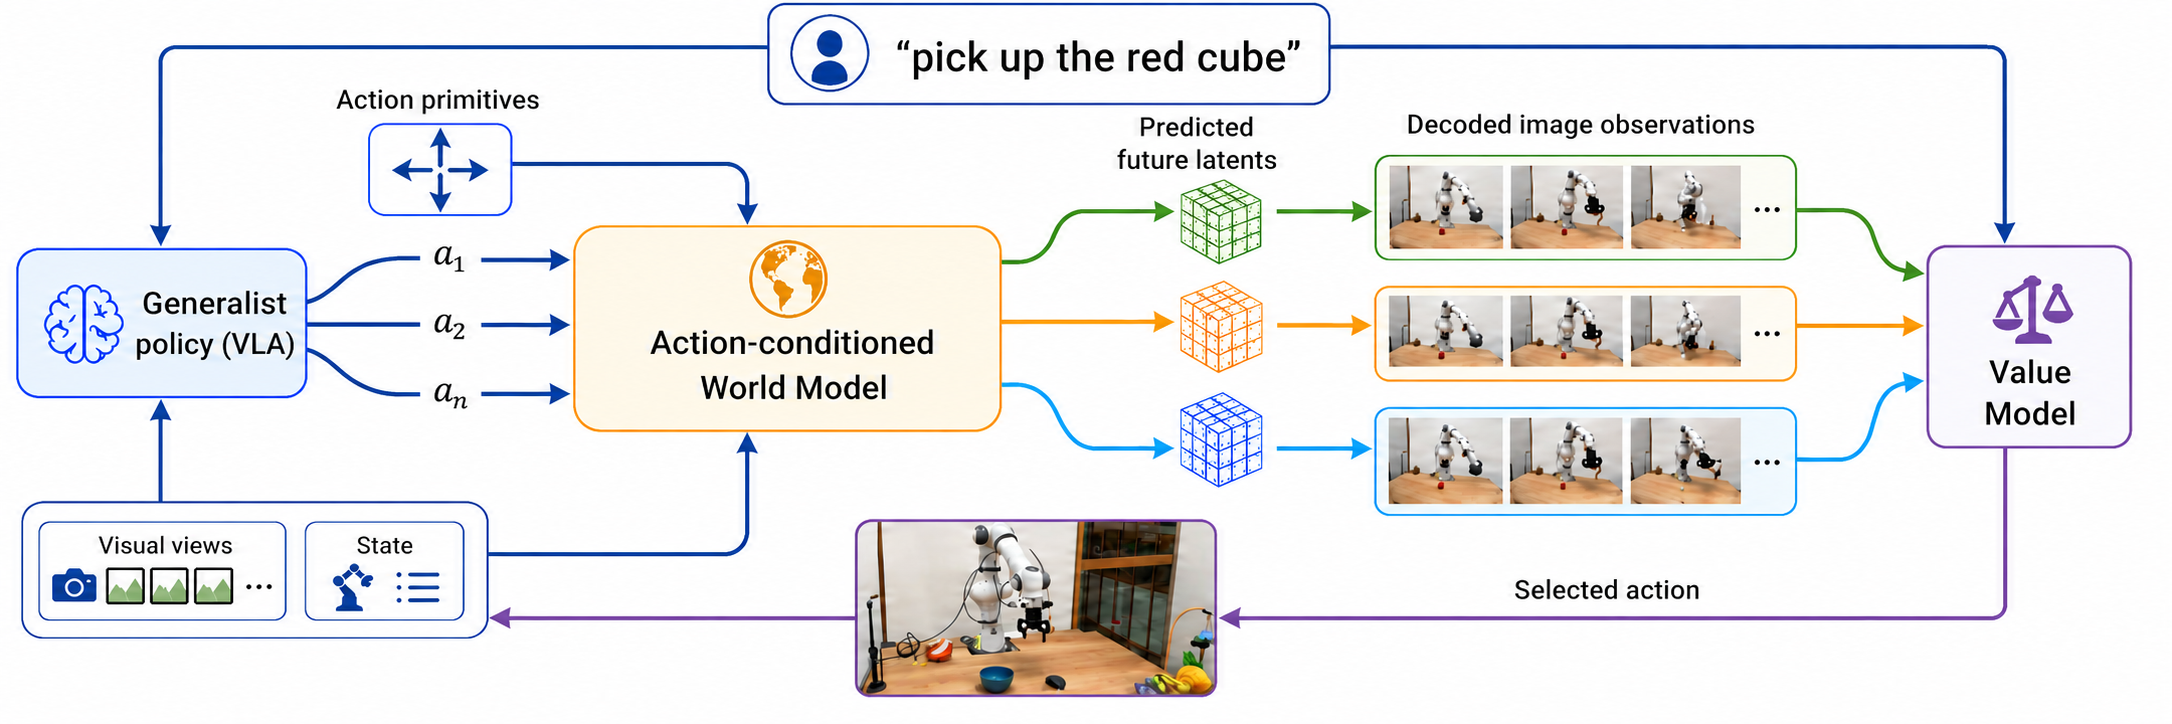
\includegraphics[width=\textwidth]{figures/dreamsteer_overview_gpt_edited_hanchen.png}
    \caption{\textbf{\coolname: deployment-time policy steering.}
    A frozen VLA policy proposes candidate action chunks, which are augmented with a small set of predefined Cartesian action primitives. A latent world model predicts future observations, and a language-conditioned value model ranks the resulting trajectories before execution. \textbf{All models are trained frozen, and no target-environment data is used during model training}.}
    \label{fig:dreamsteer}
\end{figure}